\section{Mechanik der Punktmasse und des starren Körpers}
\begin{auf}
    154
\end{auf}
Eine mit Sand gefüllte Holzkiste der Masse $M=20kg$ ist an Schnüren der Länge $l=1.2m$ aufgehängt. In die anfangs ruhende Kiste wird ein Projektil der Masse $m=10g$ geschossen, wobei es in der Kiste stecken bleibt.
\begin{enumerate}
    \item[\ref{eq:154_a}] Welche Geschwindigkeit $v$ hatte das Projektil, wenn die Kiste dadurch maximal $x=4.9 cm$ horizontal ausgelenkt wird?
    \item[\ref{eq:154_b}] Wie groß ist der in Wärme und Verformungsarbeit umgewandelte Anteil der ursprünglich vorhandenen Energie?
\end{enumerate}
\begin{figure}[h]
    \centering
    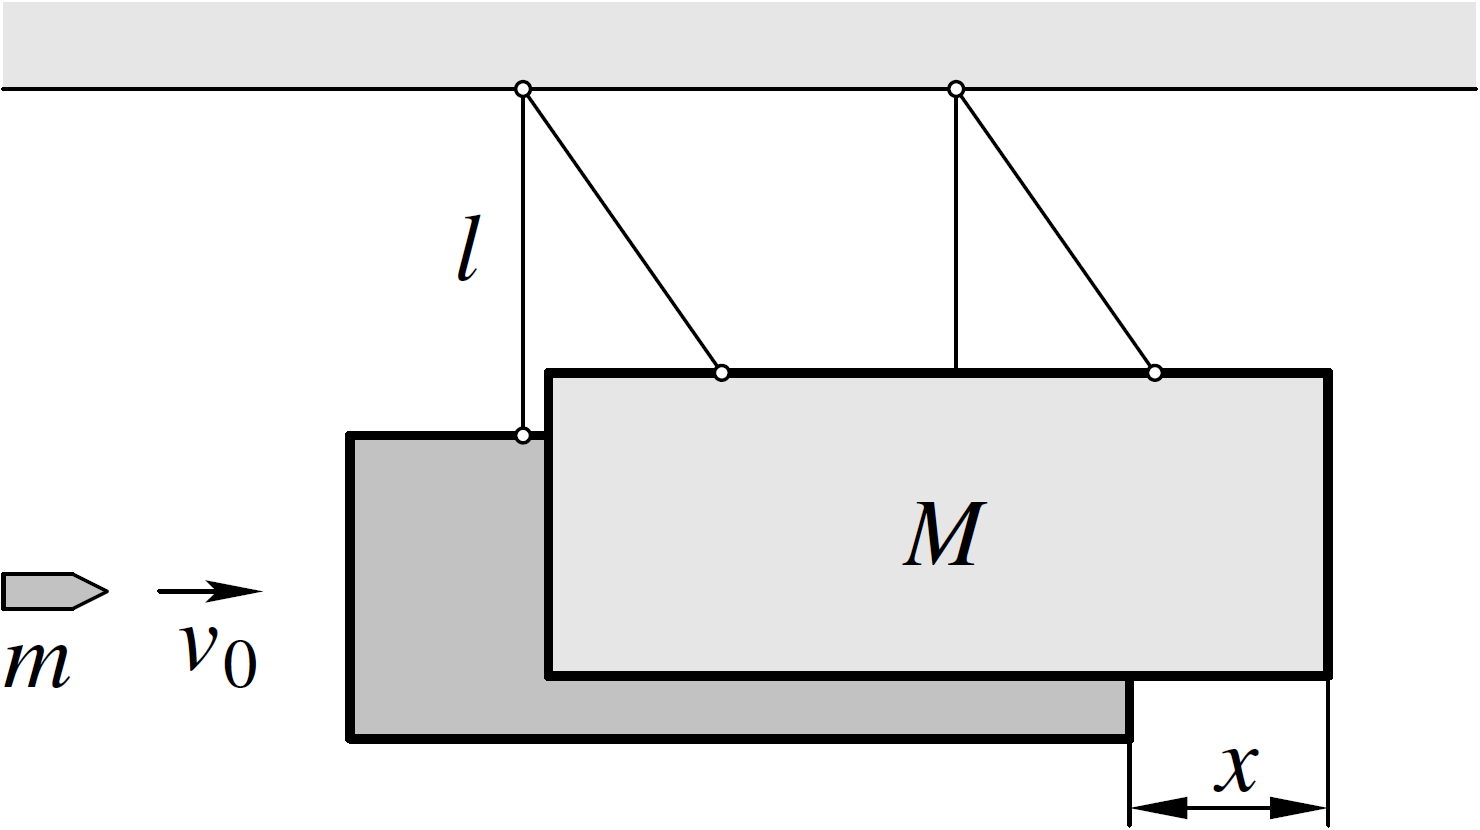
\includegraphics[width=0.7\linewidth]{images/154_0.png}
    \caption{Versuchsaufbau Aufgabe 154}
\end{figure}
Es handelt sich hierbei um einen unelastischen Stoß. Dabei hat die Masse $m$ zu Beginn die Geschwindigkeit $v$ und die Masse $M$ befindet sich anfangs in Ruhe, das heißt ihre Geschwindigkeit beträgt $0\frac{m}{s}$. Nach dem Stoß besitzen beide Massen die Geschwindigkeit $v'$.
\begin{align}
    m\cdot v &= (m+M)\cdot v'				\nonumber\\
    v&=\frac{m+M}{m}\cdot v' 				\nonumber\\
    v&=\left(1+\frac{M}{m}\right)\cdot v'	\label{eq:154_velocity0}
\end{align}
Bei der anschließenden Pendelbewegung vom hängenden Zustand 1 in den ausgelenkten Zustand 2 erfolgt eine Energieumwandlung von kinetischer Energie in potenzielle Energie. Es gilt der Energieerhaltungssatz. Dabei ist die potentielle Energie im Zustand 1 $0J$. Die kinetische Energie im Zustand 2 ist ebenfalls $0J$.
\begin{align}
    E_{kin_1}+E_{pot_1}&=E_{kin_2}+E_{pot_2}		\nonumber\\
    E_{kin_1}&=E_{pot_2}							\nonumber\\
    \frac{(m+M)\cdot v'^2}{2}&=(m+M)\cdot g\cdot h	\nonumber\\
    \frac{v'^2}{2}&=g\cdot h						\nonumber\\
    v'&=\sqrt{2\cdot g\cdot h}						\label{eq:154_velocity1}
\end{align}
Der Zusammenhang zwischen horizontaler und vertikaler Auslenkung ergibt sich aus dem Satz des Pythagoras.
\begin{figure}[h]
    \centering
    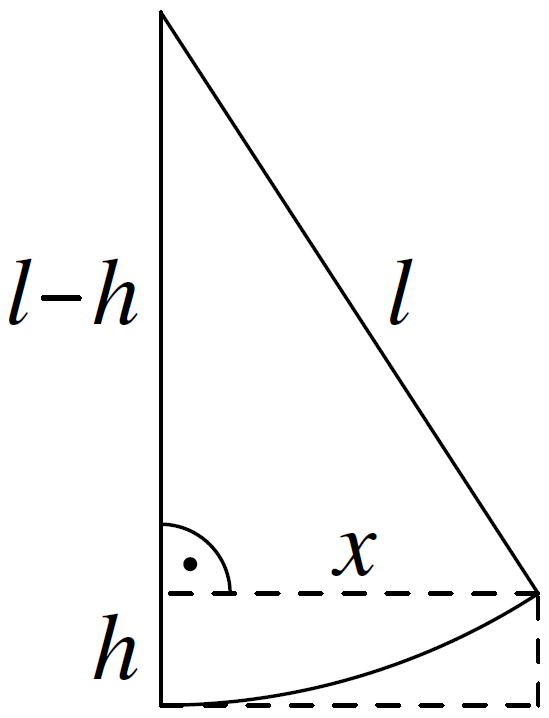
\includegraphics[height=2.5cm]{images/154_1.png}
    \caption{Skizze Pendelbewegung}
\end{figure}
\begin{align}
    (l-h)^2+x^2&=l^2		\nonumber\\
    (l-h)&=\sqrt{l^2-x^2}	\nonumber\\
    h&=l-\sqrt{l^2-x^2}		\label{eq:154_height}
\end{align}
Setzt man nun die Gleichungen \eqref{eq:154_height} und \eqref{eq:154_velocity1} in \eqref{eq:154_velocity0}, ein erhält man für die Anfangsgeschwindigkeit:
\begin{align*}
    v&=\left(1+\frac{M}{m}\right)\cdot\sqrt{2\cdot g\cdot\left(l-\sqrt{l^2-x^2}\right)}\\
    v&=\left(1+\frac{20kg}{0.01kg}\right)\cdot\sqrt{2\cdot 9.81\frac{m}{s^2}\cdot\left(1.2m-\sqrt{(1.2m)^2-(0.049m)^2}\right)}\\
    &\boxed{v=280.4\frac{m}{s}}		\tag{a} \label{eq:154_a}
\end{align*}
Um den Anteil der Energie, welcher in Wärme und Verformungsarbeit $\Delta E$ umgewandelt wurde, zu ermitteln sind die kinetische Energie vor und nach den Stoß zu betrachten. Dabei sei die Energie vor dem Stoß $E$.
\begin{align*}
    \Delta E&=\frac{m\cdot v^2}{2}-\frac{(m+M)\cdot v'^2}{2}\\
    \Delta E&=\frac{m\cdot v^2}{2}-\frac{m+M}{2}\cdot \left(\frac{m}{m+M}\cdot v\right)^2\\
    \Delta E&=\frac{m\cdot v^2}{2}-\frac{m^2\cdot v^2}{2\cdot(m+M)}\\
    \Delta E&=\left(1-\frac{m}{m+M}\right)\cdot\frac{m\cdot v^2}{2}\\
    \Delta E&=\left(1-\frac{m}{m+M}\right)E\\
    \Delta E&=\left(1-\frac{0.01kg}{0.01kg+20kg}\right)E\\
    &\boxed{\Delta E=0.9995E}		\tag{b}	\label{eq:154_b}
\end{align*}